\section{Experiments}
The experiments compare various settings of match pairs for the runtime performance of error detection.
The match pairs in all the tests are generated by the new algorithm in this paper with different $k$. 
The encodings are resolved by the SMT solver Z3 \cite{demoura:tacas08}. 

A series of experiments were conducted for six typical benchmark programs that are employed by other papers \cite{benchmark:fevs,mpptest_benchmark,DBLP:conf/kbse/HuangMM13,HuangDeadlock,DBLP:conf/ppopp/XueLWGCZZV09}. For each benchmark, the encoding was adjusted for detecting three types of errors: assertion violation, zero buffer incompatibility and deadlock. 
%The results are shown in \tableref{table:benchmarks}. 
The initial execution trace for a CTP is generated by instrumenting the MPI programs with manually written scripts and executing the programs by MPICH \cite{mpich}, a public implementation of the MPI standard. The SMT encoding is generated by the rules in the prior work \cite{DBLP:conf/kbse/HuangMM13,HuangNFM15,HuangDeadlock}.
%In precise, detecting assertion violation needs to encode the negation of user-provided assertions with respect of the computation in the program. Detecting zero buffer incompatibility needs to encode zero buffer semantics. The orphaned receive deadlock needs to encode the disjunction of the match pairs for each send for validating the potential deadlock. The assertion violation and the orphaned receive deadlock are tested under infinite buffer semantics. 
The experiments are run on a AMD A8 Quad Core processor with 6 GB of memory running Ubuntu 14.04 LTS. A time limit of 2 hours is set for each test. The test aborts the verification process if it does not complete within the time limit.

The results of the comparison are shown in \tableref{table:benchmarks}.  
The column ``Match" records the number of the generated match pairs as input to the SMT encoding. The column ``$k$" records the number as input to the algorithm in this paper. If ``$k$" is equal to the notation ``$\infty$", the match pairs are over-approximated. The columns ``EX", ``D", ``Time" and ``Impr" are measured for each of the three errors. The column ``EX" indicates whether an error exists in the tested program. The column ``D" indicates whether the error is detected or not. The column ``Time" is for both constraint generation and solving. The notation ``TO" means ``time out" (exceeding the time limit set for each test). The column ``Impr" records a decimal that represents the runtime improvement of the SMT encoding from that with the over-approximated match pairs. 
The value is computed by the simple formula in equation (4), where $\mathrm{Time}(\infty)$ is the runtime of the encoding with the over-approximated match pairs, and $\mathrm{Time}(\mathrm{k})$ is the runtime of the same encoding, where only the match pairs are generated with the input $k$. 
\begin{equation}
\mathrm{Impr} = \frac{\mathrm{Time}(\infty)}{\mathrm{Time}(\mathit{k})}
\end{equation}
According to equation (4), a higher value for $\mathrm{Impr}$ indicates a shorter runtime of the encoding where the problem instance is simpler with the match pairs generated with $k$.
The meaning of the symbol ``-" is ``unavailable": the test is not interesting for comparison.

\begin{savenotes}
\begin{table*}[t]
\begin{center}
\scriptsize
\caption{Tests on Selected Benchmarks}\label{table:benchmarks}
     \begin{threeparttable}
\begin{tabular}{|c|c|c|c|c|c|c|c|c|c|c|c|c|c|c|c|c|}
		\hline
         \multicolumn{5}{|c|}{Test Programs} & \multicolumn{4}{c|}{Assertion Violation} & \multicolumn{4}{c|}{Zero Buffer Incom\tnote{\textdagger}} & \multicolumn{4}{c|}{Deadlock}  \\ \hline
          $Name$ & \#P & \#OP &$k$& \#Match & EX & D & Time& Impr &EX&D & Time & Impr& EX &D & Time &Impr\\ \hline
          \multirow{3}{*}{\textit{Diff2DNoBa}} & \multirow{3}{*}{16}& \multirow{3}{*}{188} & 1 & 514 & No & -- &3.508s & 19.35 & Yes &  &1.749s&3.07 & Yes&$\surd$ & 3.479s& 13.50 \\ \cline{4-17}
								&				&                               & 2 & 934 & No & -- & 47.484s & 1.43 & Yes & & 3.053s& 1.76 &Yes& $\surd$& 44.060s&1.07\\ \cline{4-17}
								&				&                               & $\infty$& 1,066 & No& -- & 67.875s& 1.00 & Yes & $\surd$ &5.375s&1.00&Yes & $\surd$& 46.974s &1.00\\ \hline
								\hline
	
	 \multirow{3}{*}{\textit{DeepComm}} & \multirow{3}{*}{5}& \multirow{3}{*}{180} & 1 & 240 & Yes & $\surd$& 0.837s & 1,647& No &  & 0.875s & 291 & No & -- & --\tnote{s} & --\\ \cline{4-17}
								&				&                            & 5 & 960 & Yes & $\surd$& 10.547s & 131 & No &  & 3.056s & 83 & No& --& --\tnote{s}& --\\ \cline{4-17}
								&				& 			     & $\infty$ & 2,760 & Yes & $\surd$ & 1,379s & 1.00 & No &  & 255s  & 1.00 &No& --& --\tnote{s}& --\\ \hline
								\hline
								
	 \multirow{3}{*}{\textit{Pktuse}} & \multirow{3}{*}{5}& \multirow{3}{*}{2048} & 1 & 1,792 &Yes & $\surd$ & 180s & $>$40 & No &  & 121s & $>$59 & No&--&--\tnote{s}&--\\ \cline{4-17}
								&				& 		       &  5   &    4,828      & Yes& $\surd$ & 564s & $>$13& No &  & 449s & $>$16 &No&--&--\tnote{s}&--\\ \cline{4-17}
								&				& 		       &  $\infty$ & 99,328&Yes & -- & TO & --& No & &  TO & --&No&--&--\tnote{s}&--\\ \hline
								\hline
								
	 \multirow{3}{*}{\textit{MultiM}} & \multirow{3}{*}{3}& \multirow{3}{*}{266} & 1 & 500 & Yes  &$\surd$&10.892s& 295 & No & & 8.312s&366 & No&-- &--\tnote{s} &-- \\ \cline{4-17}
								&				&                   & 5& 1,300 & Yes& $\surd$& 24.397s & 132 & No & &17.843s & 170&No&--&--\tnote{s}&--\\ \cline{4-17}
								&				&                   & $\infty$ & 20,300 & Yes & $\surd$ & 3,218s & 1.00& No& &  3,043s& 1.00&No&--&--\tnote{s}&--\\ \hline
								\hline
								
	 \multirow{3}{*}{\textit{Mismatch}} & \multirow{3}{*}{3}& \multirow{3}{*}{800} & 1 & 204 & No &-- &--\tnote{a} & --&No & & 2.904s & 3.06&Yes&$\surd$&2.160s& 6.61\\ \cline{4-17}
								&				& 			 & 30 & 622 & No&-- &--\tnote{a} &-- & No& & 3.297s& 2.69 &Yes&$\surd$&10.061s&1.42\\ \cline{4-17}
								&				& 			 & $\infty$& 793 &No &-- &--\tnote{a} &-- & No& & 8.872s &1.00 &Yes&$\surd$&14.286s&1.00\\ \hline
								\hline
			
	 \multirow{3}{*}{\textit{Floyd}} & \multirow{3}{*}{32}& \multirow{3}{*}{528} &1& 1,928 & No&-- &29.925s & 0.97 & No &  & 89.032s & 1.02 & No&--&--\tnote{s}&--\\ \cline{4-17}
								&				& 		     & 5&1,928 & No &-- &30.621s & 0.95 & No &  & 90.908s& 1.00&No&--&--\tnote{s}&--\\ \cline{4-17}
								&				& 		     & $\infty$&1,928 &No &-- &29.043s &1.00 & No&  &91.155s &1.00 &No&--&--\tnote{s}&--\\ \hline
           
        
         
\end{tabular}
\begin{tablenotes}
\item[\textdagger] All the precise match pairs are required to witness a program zero buffer incompatible.
\item[s] SMT analysis is not launched because no potential deadlock is detected in preprocessing.
\item[a] No assertion is implemented in the program.
\end{tablenotes}
     \end{threeparttable}
\end{center}
\end{table*}
\end{savenotes}

Six typical benchmarks are tested. \textit{Diffu2DNoBa} is modified from the program \textit{Diffusion 2D}, which uses barriers to “partition” the message communication into several sections \cite{benchmark:fevs}. \textit{Diffu2DNoBa} removes the barriers from the original program. As such, deadlocks are present in the new program.

\textit{DeepComm} is a simple program with one receiver and 4 senders. In the program, the receiver issues 60 wildcard receives; each sender sends 15 messages to the receiver.
This scenario reflects the message non-determinism with 60 messages, such that the messages from different senders may race.

\textit{Pktuse} can be executed with 5 processes -- each of which randomly sends several messages to the other processes \cite{mpptest_benchmark}. The program uses wildcard receives only, therefore has a high degree of message non-determinism.

\textit{MultiM} is an extension to a program in the MCAPI library distribution \cite{DBLP:conf/kbse/HuangMM13}. The program adds extra iterations to the original program to generate longer execution trace. The assertions may be violated in possible executions.

\textit{Mismatch} implements the message communication that contains a deadlock \cite{HuangDeadlock}. No assertions are present in the program.

\textit{Floyd} implements the shortest path algorithm for all the pairs of nodes \cite{DBLP:conf/ppopp/XueLWGCZZV09}. Each node communicates only with the immediate following neighbor. 

The results show that all the errors in the benchmarks can be efficiently detected by the SMT encoding with under-approximation of the precise match pairs. The benchmarks \textit{Diffu2DNoBa}, \textit{DeepComm}, \textit{Pktuse}, \textit{MultiM} and \textit{Mismatch} show that the runtime performance is highly improved as errors are detected with a small set of match pairs. For example, the value of $\mathrm{Impr}$ is 1,647 with $k=1$ for the benchmark \textit{DeepComm}, indicating that the runtime is highly improved.
Further, the match pairs generated with $k=1$ is sufficient to detect the errors in these programs. 
For example, the encoding runs under a second for $k=1$ to find a violated assertion in the program \textit{DeepComm}, while the runtime of the same encoding with the over-approximated match pairs is more than 20 minutes. 
For the program \textit{Mismatch}, the deadlock can be detected around 2 seconds for $k=1$, while the encoding with the over-approximated match pairs needs to run 14 seconds for the same error. 

To check zero buffer incompatibility, the precise match pairs are required because a zero buffer incompatible program indicates that all possible schedules are infeasible under zero buffer semantics. 
As such, the zero buffer incompatibility for the program \textit{Diff2DNoBa} is only detected with $k=\infty$. 
On the other hand, if any schedule for a program is able to run under zero buffer semantics, the program may never be zero buffer incompatible.
As such, if a test shows that a zero buffer encoding is satisfiable for the program, then the program is proved to be zero buffer compatible. 
%This is because the test demonstrates that there is at least one feasible schedule that may occur under zero buffer semantics. 
The results show that the benchmarks excluding the program \textit{Diff2DNoBa} are zero buffer compatible by testing them with only a small set of match pairs.

For deadlock detection, a prior static analysis is launched as preprocessing to find all the potential deadlocks in a program. If no potential deadlocks are found, then the SMT encoding is not required. For example, the deadlock test for the program \textit{MuitiM} is unavailable because no potential deadlock is detected.

\begin{figure}[!h]
%\centering
\begin{minipage}{.5\textwidth}
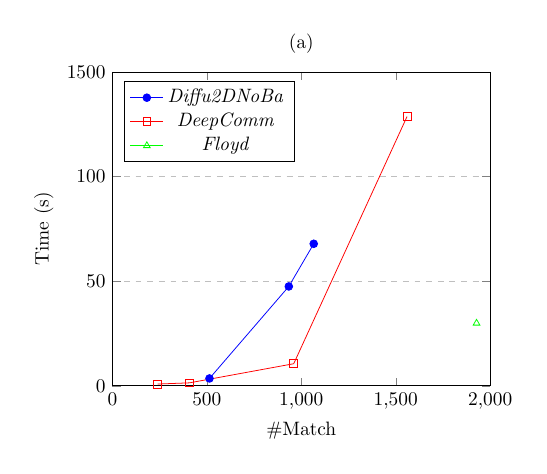
\begin{tikzpicture}[scale=0.7]
\begin{axis}[
title = {(a)},
    xlabel={\#Match},
    ylabel={Time (s)},
    xmin=0, xmax=2000,
    ymin=0, ymax=150,
    xtick={0,500,1000,1500,2000},
    ytick={0,50,100,150},
    yticklabels={0,50,100,1500},
    legend pos=north west,
    ymajorgrids=true,
    grid style=dashed,
]
 
\addplot[
    color=blue,
    mark=*,
    ]
    coordinates {
    (514,3.508)(934,47.484)(1066,67.875)
    };

\addplot[
    color=red,
    mark=square,
    ]
    coordinates {
    (240,0.837)(408,1.409)(960,10.547)(1560,128.681)
    };

\addplot[
    color=green,
    mark=triangle,
    ]
    coordinates {
    (1928,29.925)
    };
    \legend{\textit{Diffu2DNoBa},\textit{DeepComm},\textit{Floyd}}
 
\end{axis}
 
\end{tikzpicture}
\end{minipage}
\begin{minipage}{.5\textwidth}
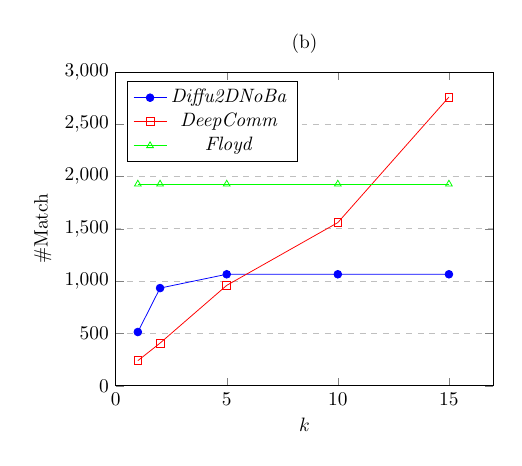
\begin{tikzpicture}[scale=0.7]
\begin{axis}[
   title = {(b)},
    xlabel={$k$},
    ylabel={\#Match},
    xmin=0, xmax=17,
    ymin=0, ymax=3000,
    xtick={0,5,10,15},
    xticklabels={0,5,10,15,20,25,30,35,40,$\infty$},
    ytick={0,500,1000,1500,2000,2500,3000},
    legend pos= north west,
    ymajorgrids=true,
    grid style=dashed,
]
 
\addplot[
    color=blue,
    mark=*,
    ]
    coordinates {
    (1,514)(2,934)(5,1066)(10,1066)(15,1066)
    };
    
\addplot[
    color=red,
    mark=square,
    ]
    coordinates {
    (1,240)(2,408)(5,960)(10,1560)(15,2760)
    };
    
\addplot[
    color=green,
    mark=triangle,
    ]
    coordinates {
    (1,1928)(2,1928)(5,1928)(10,1928)(15,1928)
    };
    \legend{\textit{Diffu2DNoBa},\textit{DeepComm},\textit{Floyd}}
\end{axis}
\end{tikzpicture}
\end{minipage}
\caption{(a) The time of assertion violation detection of varying the number of match pairs. (b) The number of match pairs of varying the input $k$.}
\label{fig:relation}
\end{figure}


To evaluate how the input $k$ impacts the number of the generated match pairs and the runtime cost of SMT encoding, the diagrams in \figref{fig:relation} show the relations for three benchmarks. The curves in \figref{fig:relation} are depicted with both the experimental data in \tableref{table:benchmarks} and additional test data if needed. \figref{fig:relation} (a) illustrates the relation between the number of the generated match pairs and the runtime for assertion violation detection. For the programs \textit{Diffu2DNoBa} and \textit{DeepComm}, the relations both show that the runtime increases exponentially as the number of match pairs grows. This observation demonstrates that the error detection is scalable only if the number of match pairs is less than a threshold. For example, detecting assertion violation for \textit{Diffu2DNoBa} is able to scale well with a set of match pairs where the size is less than 1,000.
Note that the program \textit{Floyd} only displays a single point in the diagram as the number of the generated match pairs is identical for each test.


\figref{fig:relation} (b) shows the relation between the input $k$ and the number of the generated match pairs. For the program \textit{DeepComm}, the relation grows stably where the number of the generated match pairs is proportional to $k$. 
This is because \textit{DeepComm} frequently sends messages back and forth between any two processes. The algorithm in this paper works well for this type of programs because the match pairs can be generated gradually as $k$ increases.

In contrast, the relation for the program \textit{Diffu2DNoBa} has a sharp growth between $k=1$ and $k=2$. After that, the relation grows stably until the number of the generated match pairs reaches the limit, which represents the largest set of match pairs generated by the algorithm. 
Another example is the program \textit{Floyd}, where the number of the generated match pairs is identical for every setting of $k$. 
Both programs show that each process only receives few (possibly a single) messages from any sender.
Therefore, the new algorithm sections each process into few sections given a lower $k$. 
The new algorithm does not scale well for this type of programs.


